%!TEX root = ../../main.tex


\begin{figure}[!htb]
\centering
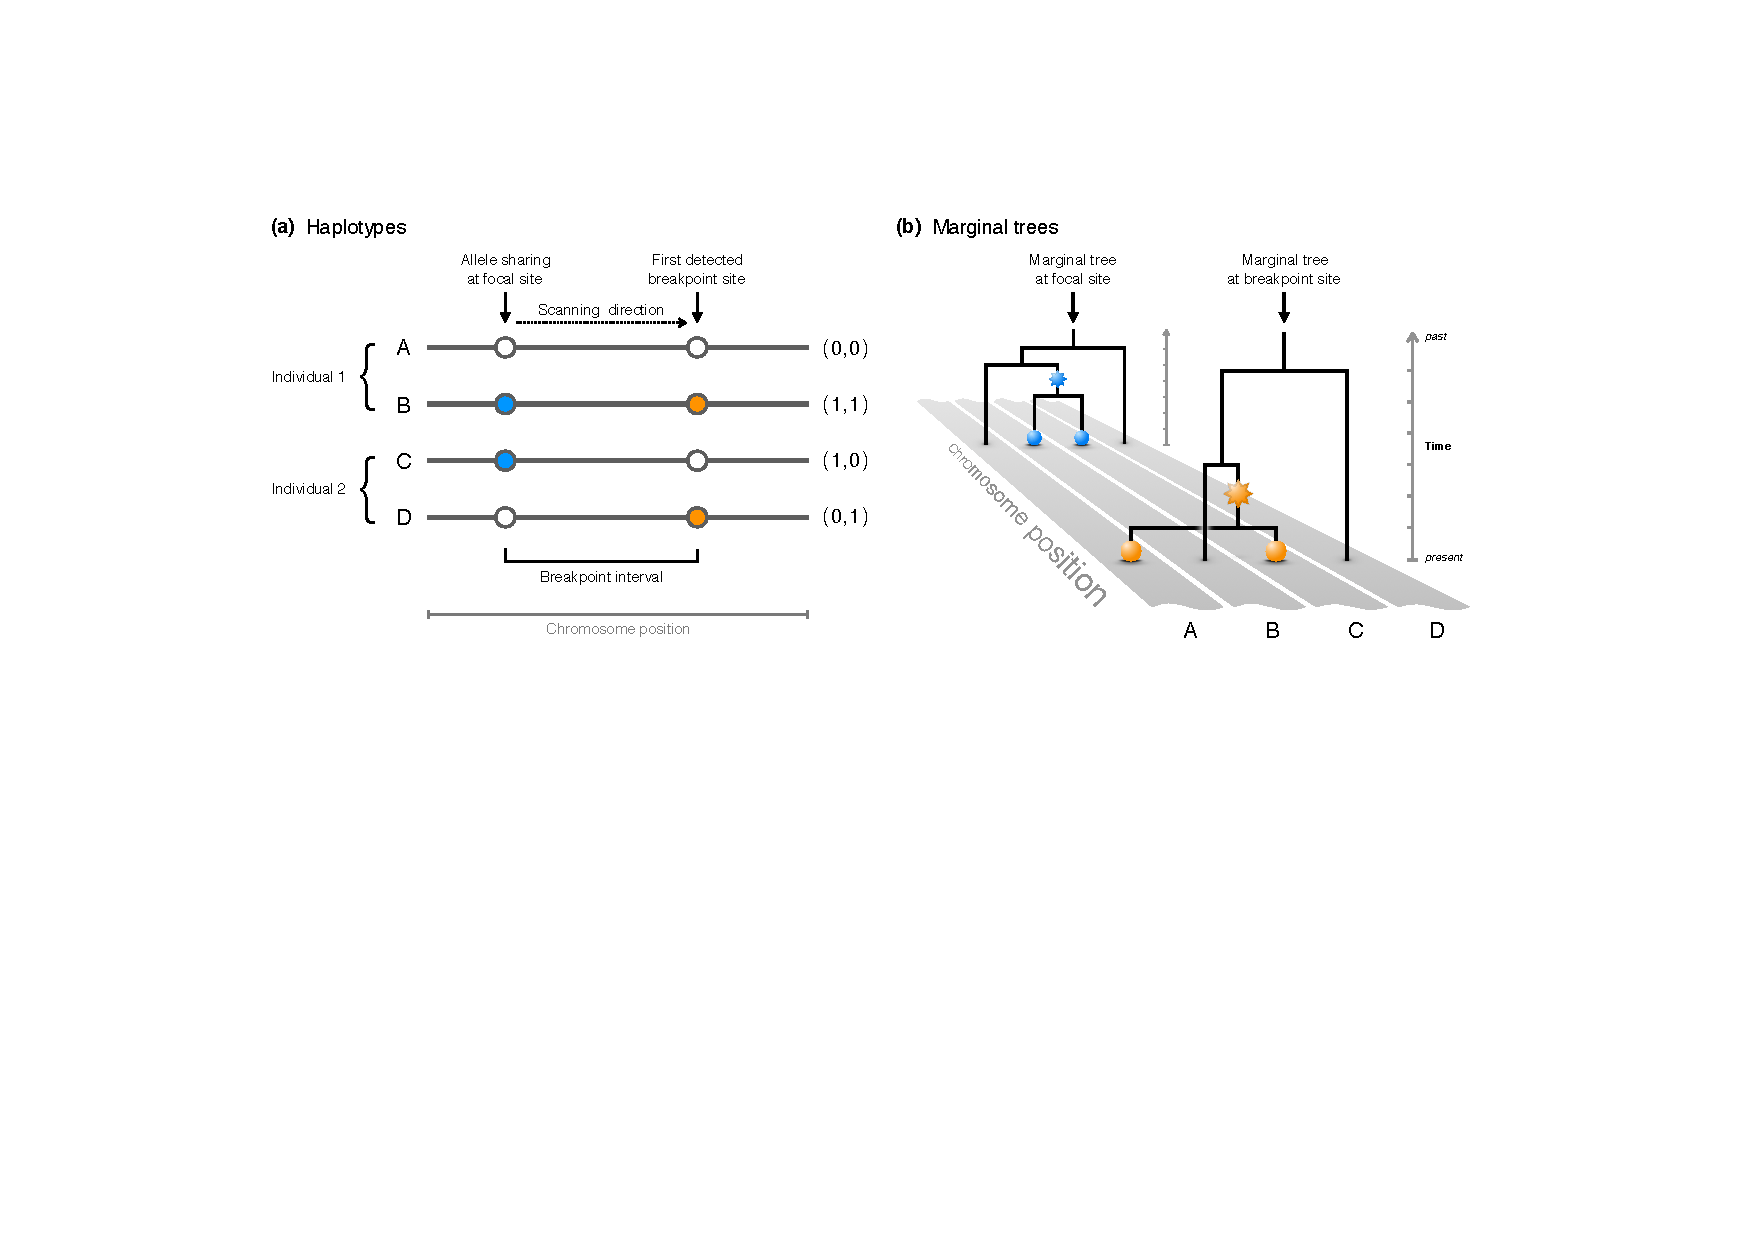
\includegraphics[width=\textwidth]{./img/ch3/info_fgt_new}
\Caption{Breakpoint detection using the four-gamete test (FGT)}
{Panel~\textbf{(a)} shows the \n{4} haplotypes (gametes) in a pair of \n{2} diploid individuals (\emph{horizontal lines}).
The focal allele (\emph{blue}) on haplotypes $B$ and $C$ is shared by both individuals.
A breakpoint interval is detected if all \n{4} possible allelic state configurations are observed at \n{2} variant sites along the sequence.
Beginning at a given focal site, which is heterozygous in both individuals, the sequences are scanned independently to the left and right hand-side (only right hand-side is shown) until a breakpoint is inferred.
The interval delimits the region in which at least \n{1} recombination event must have occurred in the history of the sample (given the assumptions of the infinite sites model).
The \n{4} allelic state configurations are shown on the \emph{right} to each sequence.
The alleles are shown at the \n{2} breakpoint sites; indicated as ancestral (\emph{hollow} circle) and derived state (\emph{solid}).
Note that the order of gametes is ignored.
Panel~\textbf{(b)} shows the corresponding marginal trees at the focal site and the detected breakpoint, where \emph{stars} indicate a mutation event and \emph{spheres} the derived alleles.}
{fig:info_fgt}
\end{figure}
